\documentclass[12pt]{article}
\usepackage{amsfonts, epsfig}
\usepackage[authoryear]{natbib}
\usepackage{graphicx}
\usepackage{fancyhdr}
\pagestyle{fancy}
\lfoot{\texttt{comsm0094.github.io}} \lhead{LC\&B - 01.6 Recording from the brain - Conor} \rhead{\thepage} \cfoot{}
\begin{document}

\section*{Recording from the brain}

In the earliest days of philosophy and science there was a belief that
we could make progress in understanding the brain by thinking about
thought, by a complex process of structured introspection. It is
likely that this still has a role in our broad subject, but it is
equally clear that the fact of science, the facts we can discover by
observing the dynamics of neural matter, are vital to understanding
the brain. The tools of neuroscience were for a long time very crude;
as we saw, the main approach was to study patients while they were
alive and then dissect them after they died. Now, though, we have a
diversity of approaches to recording the dynamics of neural matter.

The ideal, obviously, would be to record all the voltage changes for
all the neurons in the brain and, probably, the different levels of
different chemical. That isn't possible and any approach to recording
from the brain is a compromise between spatial and temporal resolution
and between the degree of intervention: at one extreme \textsl{in
  vitro} experiments are done on slices of brain that have been
removed from an animal, typically one that has been killed as part of
the experiment, these experiments can record the voltage inside the
neuron an sub-milisecond resolutions. At the other extreme
\textsl{electroencephalography} is completely non-invasive, you might
end up with conductive gel on your hair but beyond that, there is no
ill-effect or annoyance to the subject, but the date is very noisy and
is a sort of smeared out average of the activity of lots of synapses.

This document is intended only as a quick tour of some recording
techniques: the speed at which the field is advancing and the vast
diversity of approaches means any description is only very partial and
slightly out-of-date.

\subsection*{In vitro electrophysiology}

In \textsl{in vitro} electrophysiology a small piece of the brain is
removed and placed in a dish where it is kept alive by careful control
of chemical composition and oxygen level of the fluid the slice is
bathed in. An electrode is then used to record from the cell; this
electrode is often a thin glass tube filled with salty water and it
sort of ``sucks'' onto the cell making a seal, see
Fig.~\ref{fig:patch}. This approach typically gives a complete
recording of the voltage inside in the cell; it can be used, for
example, to measure the size of an PSP, the dendritic voltage change
at a synapse.

Slices are usually made in a way that preserves as much of the
neurites, the axons and dendrites, as possible; this is easier in some
parts of the brain than others, the hippocampus for example lends
itself to \textsl{in vitro} approaches because it has a very laminar
structure and a lot of what we know about synapses was discovered in
hippocampus. However, the key point is that these neurons are not in
their natural environment, they will have damaged neurites, the
chemical and temperature environment is not normal and their input is
nothing like what it would be in the brain.

\begin{figure}
  \begin{center}
    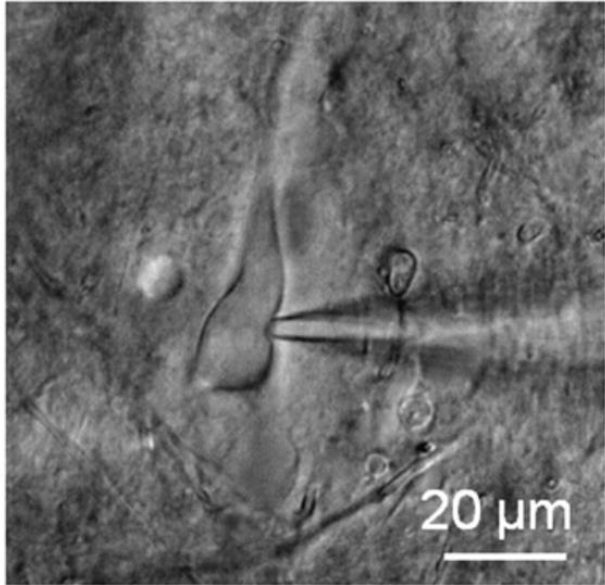
\includegraphics[width=6cm]{patch.png}
    \end{center}
  \caption{\textbf{Patched cell}: here an electrode has been \textsl{patched clamped} onto a cell to record its internal voltage. [figure from Ding, S., Mattam, S. G. \& Zhou F. M. (2011)]\label{fig:patch}}
\end{figure}

One nice approach, which has been used a lot in studying the retina,
is to lay the slice directly only an array of electrodes. This does
not give \textsl{intracellular data}: the electrodes record from
outside the cell, giving \textsl{extracellular data}, so the data are
spike times rather than voltages, but the density of electrodes that
are possible does give a very complete picture of the network
activity, albeit in this weird context.

\subsection*{In vivo electrophysiology}

The \textsl{vitro} in \textsl{in vitro} means glass, referring I think
to the glass dish the brain slice is placed in. In contrast, the
\textsl{vivo} in \textsl{in vivo} means living and \textsl{in vivo}
electrophysiology is performed using living animals, either
anesthetized or awake and behaving. To do this an electrode is placed
in the animals brain; in the anesthetized preparation a hole is cut in
the brain, \textsl{trepanation}, and the electrode is inserted through
that, or, in the awake behaving preparation, a \textsl{head stage} is
mounted on the head covering and sealing up a hole in the skull. In
the past the electrode was moved until the activity it recorded showed
it was near a neuron; these days though silicon probes can be
used. Silicon probes are made using processes similar to those used to
manufacture chips and have hundreds of recording sites; in this case
the experimenter will rely on at least some of the recording sites
being near the neurons.

In an \textsl{in vivo} experiment the electrode is outside the neuron
so only the spikes are recorded and typically, spikes from more than
one neuron are mixed together. A set of algorithms called
\textsl{spike sorting} are used to assign spikes to different
neurons. The accuracy of spike sorting is often debated; with silicon
probes spikes are often recorded, with different amplitudes, by
different recording sites, something that was already possible, but in
a much more limited way, with simpler electrodes; this allows a sort
of triangulation to be performed in spike sorting, making it more
accurate for silicon probes, however, the amount of sorting involved
with silicon probes, given their vast number of recording sites, means
the debate about how to best spike sort is as heated as ever.

The advantage of \textsl{in vivo} electrophysiology is that you can
record from the brain in a more natural state; however, the need to
tether the electrode to the recording equipment in the awake behaving
preparation limits the experiments that can be performed. Furthermore,
the data recorded gives spikes, not voltages and spiking activity
rather than synaptic activity. Although the number of neurons that can
be recorded has increased a huge amount over the last few years, it is
still a long way from recording whole brain activity. It is a highly
invasive procedure, there are animal welfare concerns and, except in
very limited circumstances related to medical treatment, it is not
possible to record from humans. Nonetheless \textsl{in vivo}
electrophysiology has been one of the main tool of neuroscience over
the last 50 years and has been the source a lot of the progress that
has been made, see as just one example Fig.~\ref{fig:place}


\begin{figure}
  \begin{center}
    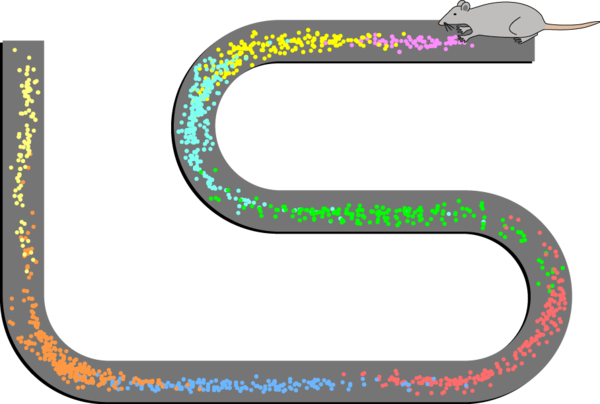
\includegraphics[width=8cm]{place_cells.png}
    \end{center}
  \caption{\textbf{Place cells}. Here each color of dot corresponds to a different neuron and the dots are placed on the maze in the location the rat was in when a spike in one of the eight neurons was fired. It shows clear evidence of place cells, with different cells firing in different locations. [figure from wikipedia]\label{fig:place}}
\end{figure}

\subsection*{Calcium imaging}



\subsection*{Summary}

\end{document}

